\subsection{Source-Evidence Development Test}
\label{app:docred_v2}
A separate version retains dual-strategy generation and the four-action scheduler, and adds document-scoped source constraints. Each candidate marks a concrete record as supported, contradicted, or insufficient. The compiler validates an exact quote in a numbered original sentence and records its character offsets. Hypothetical augmentation clauses cannot supply evidence. Insufficient evidence causes abstention. Conflicting support and contradiction also cause abstention; type compatibility alone cannot cancel a source contradiction.
For this version, let $V(g;R)$ be the set of nonconflicting violations and $N$ the initial record count (with denominator one for an empty input). We use $G(g;R)=1-|V(g;R)|/N$ and coverage $C$ over the initial records. The graph-change term compares both graphs under the updated rules:
\begin{align}
r_t={}&0.5\left[G(g_{t+1};R_{t+1})-G(g_t;R_{t+1})\right] \nonumber\\
&+0.5(C_{t+1}-C_t)-0.004a_t \nonumber\\
&-0.00002d_t-|V_{\mathrm{edit},t}|/N,
\end{align}
where $a_t$ counts acquired responses, $d_t$ counts removed records, and $V_{\mathrm{edit},t}=V(g_{t+1};R_{t+1})\setminus V(g_t;R_{t+1})$. Thus acquisition can reveal a violation without being charged for creating it. A two-record synthetic counterexample changes the discounted acquire--repair return from $-0.266519$ to $0.483481$ at discount $0.95$. This is an accounting check, not an empirical quality gain. Source support is still a model judgment; quote validation does not prove its meaning.
Before calls, we fix the first ten development pairs (20 documents). Each pair contains one reference graph and one reference graph with added endpoint or relation substitutions, numbering $\lceil0.2|G^*|\rceil$. References are used in construction and scoring, not in prompts, observations, or reward. The observations contain 14 public summaries and an action mask; they are not asserted to be a sufficient Markov state. Each episode allows four response acquisitions, two per strategy, and ten steps. The removal operator retains the emptying guard.
\begin{table}[t]
\centering
\caption{Source-evidence development diagnostics on ten fixed document pairs. F1 and preservation are episode means. Lost counts removed reference facts. No learned policy is evaluated.}
\label{tab:docred_source_pilot}
\small
\begin{tabular}{lrrr}
\hline
Schedule & F1 (\%) & Preserved (\%) & Lost \\
\hline
Stop & 94.42 & 100.00 & 0 \\
Acquire then repair & 94.59 & 98.34 & 4 \\
Repair when feasible & 91.63 & 93.51 & 18 \\
Uniform feasible & 94.42 & 100.00 & 0 \\
\hline
\end{tabular}
\end{table}
The 40 outputs require 40 actual Gemma requests. They compile to 357 type rules, 61 source-support rules, and 6 source-contradiction rules. Source constraints trigger removals in 4 of ten episodes. The pre-call expansion gate requires this in at least two episodes and at least one fixed schedule to improve mean reference F1 while preserving at least 99\% of reference facts.
The development gate is not met, so this version is not expanded to learned-policy training or held-out evaluation.
These results measure reference recovery and removal of injected items. Independent assessment of natural relations and edits remains pending. Cached schedule replay makes zero API calls; generation requests are counted separately.
\begin{figure*}[t]
\centering
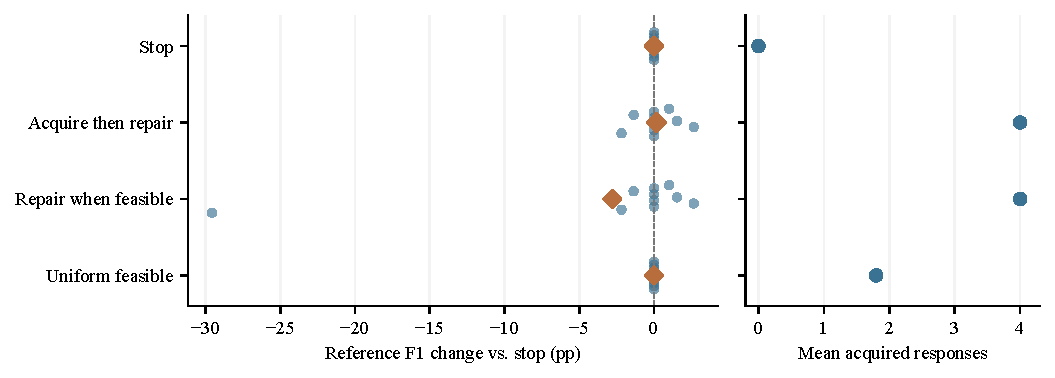
\includegraphics[width=0.94\textwidth]{figure/experiments/docred_source_pilot.pdf}
\caption{Source-evidence development replay. Small points show ten episode-level F1 changes from stop; diamonds show their mean. The right panel shows cached response acquisitions.}
\label{fig:docred_source_pilot}
\end{figure*}
